\documentclass[UTF8,fontset=fandol,a4paper,10.5pt]{ctexart}

\usepackage[margin=2.2cm,top=2.3cm,bottom=2.2cm]{geometry}
\usepackage{graphicx}
\usepackage{booktabs}
\usepackage{tabularx}
\usepackage{array}
\usepackage{float}
\usepackage{caption}
\usepackage{enumitem}
\usepackage[hidelinks]{hyperref}
\hypersetup{pdftitle={AirHust 2026 级梯队任务书},pdfauthor={AirHust 团队}}

\captionsetup{font=small,labelsep=quad}
\renewcommand{\arraystretch}{1.25}
\setlength{\parindent}{2em}
\setlength{\parskip}{2pt}

\ctexset{
  section={
    name={,、},
    number=\chinese{section},
    format=\Large\bfseries\heiti,
    aftername={},
    beforeskip=12pt,
    afterskip=8pt
  },
  subsection={
    number=\arabic{section}.\arabic{subsection},
    format=\large\bfseries\heiti,
    aftername=\quad,
    beforeskip=9pt,
    afterskip=5pt
  }
}

\begin{document}
\pagestyle{plain}

% ---------------- 封面 ----------------
\begin{titlepage}
  \centering
  \vspace*{3.2cm}

  {\zihao{1}\bfseries\heiti AirHust 2026 级梯队任务书\par}

  \vspace{1.0cm}
  {\zihao{3}\heiti 无人机仿真综合任务\par}

  \vfill

  \begin{tabular}{rl}
    {\heiti 项目：} & 梯队选拔任务 \\[8pt]
    {\heiti 编制：} & AirHust 团队 \\
  \end{tabular}

  \vspace{1.6cm}
  {\zihao{4} 2026 年 10 月\par}
\end{titlepage}
\setcounter{page}{1}

% ---------------- 正文 ----------------
\section{任务概述}

梯队选拔为综合性任务，参与者可选择完成其中部分或全部内容。评审既看重全面能力，也欣赏在某一方向有专长的同学，请根据自身情况合理规划。

\section{任务地图}

\subsection{场地规格}

\begin{enumerate}[label=（\arabic*）,leftmargin=3.2em,itemsep=3pt]
  \item 任务地图为 38\,$\times$\,8 的矩形区域，从左至右划分为五个功能区：避障区、穿门区、穿环区、识别区与降落区。场地下方设有通道，可供选择路径。
  \item 闯关顺序不作强制要求，参与者可自由选择。
  \item 图示坐标仅供参考。实际测试中，起飞点、降落点与墙体坐标准确；柱子、圆环、方框和门可能存在 10--20\,cm 的浮动；识别区目标在该测试范围内随机摆放。
\end{enumerate}

\begin{figure}[H]
  \centering
  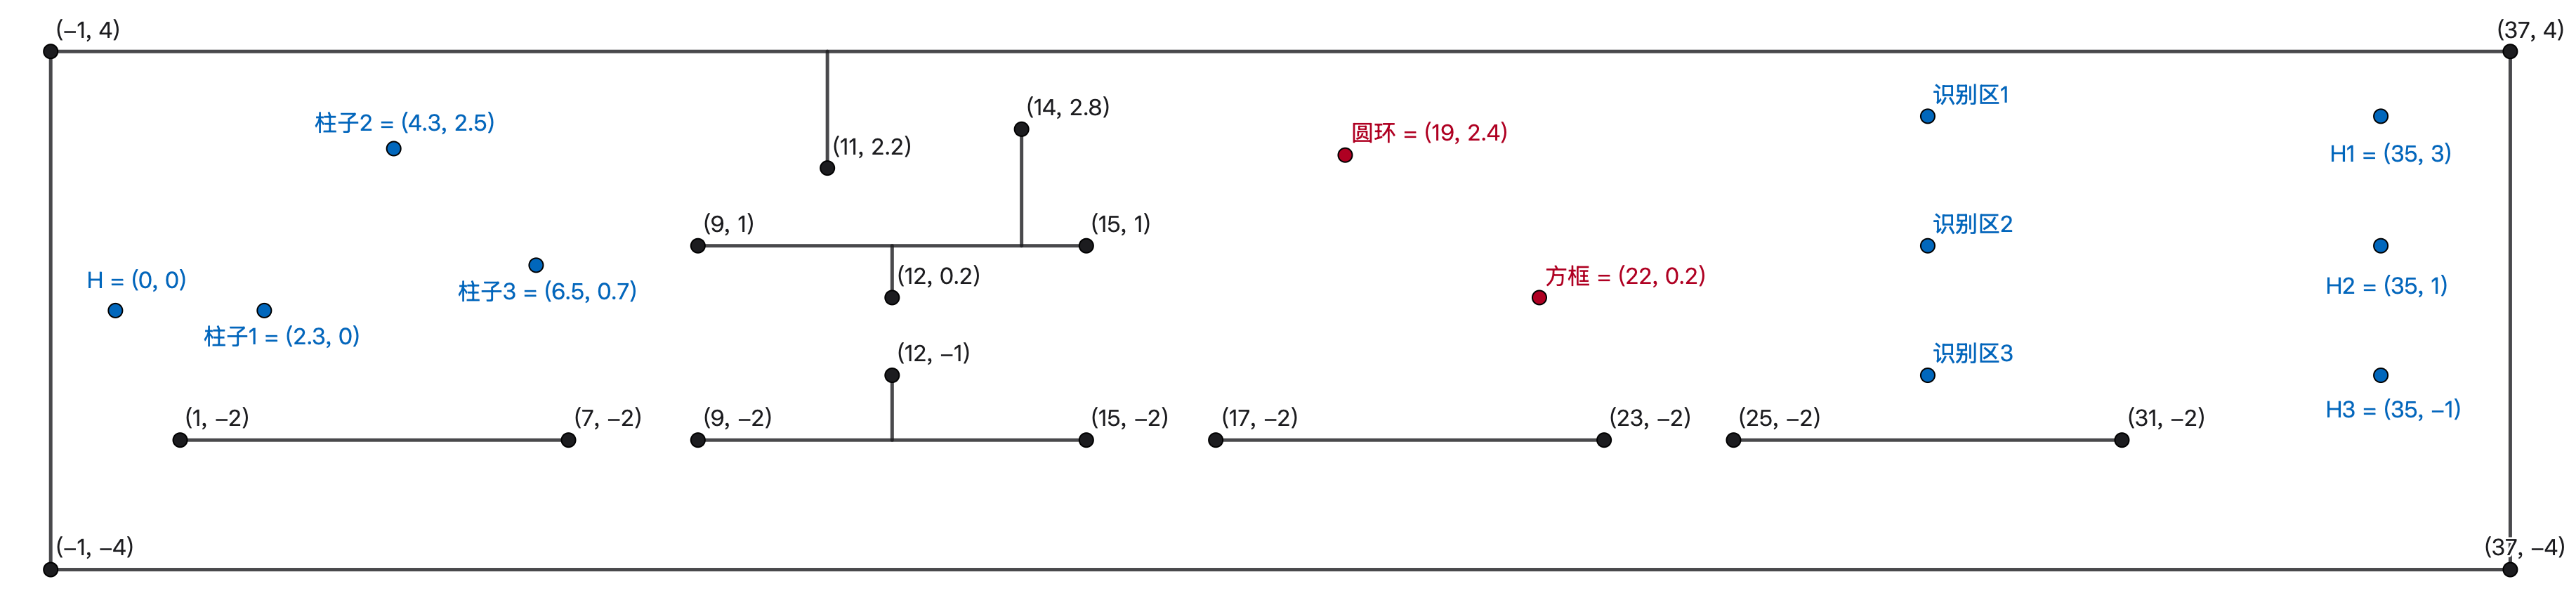
\includegraphics[width=0.95\textwidth]{figures/arena_map.png}
  \caption{任务地图与参考坐标}
  \label{fig:arena}
\end{figure}

\section{任务内容与评分}

以下六项任务的分值独立计算。

\subsection{起飞任务}

\textbf{任务要求：}起飞后悬停于 1.5 米高度，保持约 10 秒，随后进入后续任务阶段。

\textbf{评分标准：}成功起飞并稳定悬停至规定时间得 20 分；仅完成起飞得 10 分；未能完成得 0 分。

\subsection{避障任务}

\textbf{任务要求：}在不发生碰撞的前提下穿越障碍区域，并在答辩中说明所使用的避障算法。

\textbf{评分标准：}成功穿越障碍区域得 30 分；每碰撞一次障碍柱扣 5 分，每碰撞墙壁一次扣 10 分；未能完成得 0 分。

\subsection{穿门任务}

\textbf{任务要求：}选择并成功穿越指定门型结构，答辩时需阐述穿门策略与算法设计。

\textbf{评分标准：}穿越单中心门得 40 分，穿越双侧门得 50 分；每碰撞门体或墙壁一次扣 5 分；未能完成得 0 分。

\subsection{穿环任务}

\textbf{任务要求：}依次穿越指定的圆环与方框结构。

\textbf{评分标准：}每成功穿越一个结构（圆环、方框）得 50 分；如发生碰撞，该结构得分减半；未穿越得 0 分。

\subsection{识别任务}

\textbf{任务要求：}在识别区内巡航搜索，找出三个目标物（随机数字、字母与二维码），并在任务结束后于指定话题 \texttt{/target} 中输出其内容及世界坐标系中的位置。

\textbf{评分标准：}每正确识别一个目标并准确输出内容与位置得 50 分，其中内容正确 20 分、位置正确 30 分；未识别得 0 分。

\subsection{降落任务}

\textbf{任务要求：}准确识别起飞点下方色块的颜色，并在降落区中精准降落在对应颜色的靶标上。

\textbf{评分标准：}降落在靶标上但颜色识别错误得 30 分；降落位置与颜色均正确得 50 分。

\section{评分汇总}

\begin{table}[H]
  \centering
  \caption{各项任务满分汇总}
  \begin{tabularx}{0.92\textwidth}{|X|c|c|}
    \hline
    \heiti 任务 & \heiti 满分 & \heiti 说明 \\ \hline
    起飞 & 20 分 & 悬停 1.5 米约 10 秒 \\ \hline
    避障 & 30 分 & 碰撞按次扣分 \\ \hline
    穿门 & 50 分 & 以双侧门计 \\ \hline
    穿环 & 100 分 & 圆环、方框各 50 分 \\ \hline
    识别 & 150 分 & 三个目标，每个 50 分 \\ \hline
    降落 & 50 分 & 位置与颜色均正确 \\ \hline
    合计 & 400 分 &  \\ \hline
  \end{tabularx}
\end{table}

\section{时间安排}

任务提交与答辩时间待定，确定后另行通知。

\vfill

\begin{flushright}
  AirHust 团队\\
  2026 年 10 月
\end{flushright}

\end{document}
